\chapter{SOA - Software Oriented Architecture}
\section{Definizione}
SOA (Architettura orientata ai servizi) è \textbf{uno stile architettonico}, che si concentra su elementi discreti riutilizzabili chiamati \textbf{servizi}, invece che su un design monolitico, per costruire le applicazioni.
\begin{figure}[H]
    \centering
    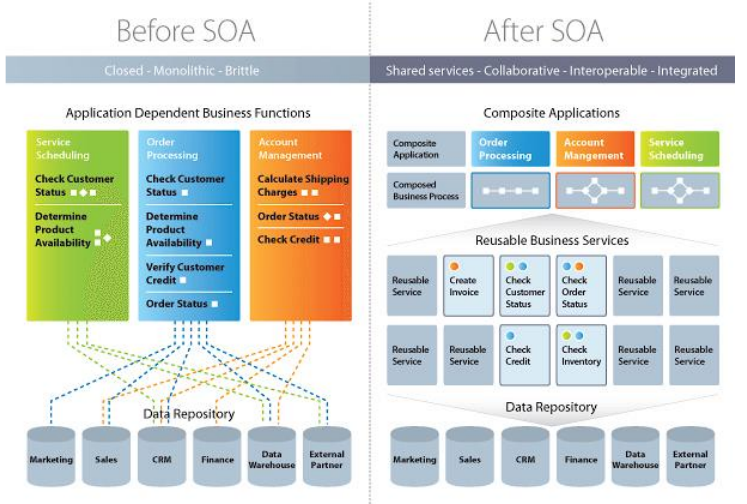
\includegraphics[scale=0.6]{figures/Schermata_20260513_102839.png}
\end{figure}

\section{Elementi fondamentali di SOA}
\subsection{Componenti}
\begin{itemize}
    \item \textbf{Servizio}: unità funzionale autonoma che esegue una funzione specifica.
    \item \textbf{Descrizione del servizio}: documento che definisce l'interfaccia, le operazione e i parametri di un servizio.
\end{itemize}

\subsection{Ruoli}
\begin{itemize}
    \item \textbf{Service Registry}: catalogo che conserva le descrizioni dei servizi, gli endpoint(URL) e le informazioni di binding (protocolli supportati, formati dei dati).
    \item \textbf{Service Provider}: chi crea un servizio e ne pubblica la descrizione nel registry.
    \item \textbf{Service Requestor}: chi consulta il registry per trovare un servizio adatto e lo invoca.
\end{itemize}

\section{Servizi}
\subsection{Definizione Informale}
Un servizio è un'entità software \textbf{indipendente} che può essere \uline{scoperta e invocata da altri sistemi software attraverso una rete}.

\subsection{Definizione Formale}
Un servizio Web è un'\textbf{applicazione software}
\begin{itemize}
    \item Identificata da un \textbf{URI}.
    \item Ha interfacce in grado di essere \uline{definite, descritte e scoperte}.
    \item Supporta \textbf{interazioni dirette} con altri sistemi software per mezzo di \uline{messa e protocolli basati su internet}
\end{itemize}

\subsection{Cosa fa un servizio?}
Ogni servizio deve:
\begin{itemize}
    \item Fornire le proprie funzionalità ai richiedenti (che possono assere altri servizi).
    \item Descrivire le sue funzionalità da scoprire e selezionare.
    \item Essere accessibile attraverso l'uso di protocolli rete noti.
    \item Supportare la collaborazione con altri servizi per fornire soluzioni complesse.
    \item Rispondere alle esigenze aziendali dei client e ai requiiti del dominio.
    \item Garantire un livello di qualità di servizio.
\end{itemize}

\subsection{Composizione dei servi}
Una \textbf{composizione} è un \uline{insieme di servizi interconnessi} che, presi nel loro insieme, costituiscono a loro volta un nuovo servizio, riutilizzabile in altre composizioni.

Due servizi \textbf{sono interconnessi} \uline{quando almeno uno dei 2 richiama la funzionalità esposta dall'altro attraverso la sua interfaccia (endpoint, API)}.

Perchè la composizione funzioni, è necessaria la \textbf{compatibilità} tra i servizi: i servizi devono parlare la stessa lingua sia \textbf{sintatticamente} (stessi formati di messaggio, stessi tipi di stato) sia \textbf{semanticamente} (stesso significato dei dati scambiati).

Per questo \uline{ogni provider} deve esporre \textbf{un'interfaccia pubblicata}, descritta in modo formale e accessibile a chi vuole consumarla.

Quando un composizione esprime un \textbf{flusso di lavoro} coordinato \uline{con un ordine di esecuzione, condizioni e dipendenze tra i servizi} parliamo di \textbf{processo di business}.

\section{Business Process}
\subsection{Definizione}
Un \textbf{business process} è un workflow strutturato di attivitò correlate, eseguite da \textbf{persone e applicazioni}, con l'obiettivo di ottenere un \textbf{risultato ben definito}.

I processi vengono realizzati tramite \textbf{composizione dei servizi}, in cui ogni attivitò è implementata come un servizio software coordinato all'interno di un flusso.

\begin{figure}[H]
    \centering
    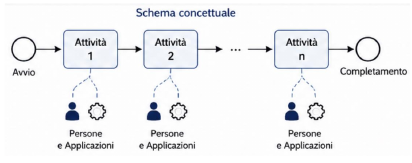
\includegraphics{figures/Schermata_20260513_121514.png}
\end{figure}

\subsection{Caratteristiche}
\begin{itemize}
    \item Può contenere \underline{condizioni definite} che ne determinano l'avvio e \underline{uscite definite} al suo completamento.
    \item Può comportare interazioni \underline{formali} o relativamente \underline{informali} tra i partecipanti (umani e software).
    \item Può contenere una serie di attività \underline{automatizzate} e/o \underline{manuali}.
    \item È \underline{distribuito} e personalizzato al di là dei confini \underline{all'interno delle organizzazioni} e \underline{tra di esse}, e spesso si estende a più applicazioni con piattaforme tecnologiche diverse.
    \item Ha una \underline{durata} che \underline{può variare notevolmente}.
    \item Di solito è di \underline{lunga durata}. 
    
    Una singola istanza può durare mesi o addirittura anni.
\end{itemize}

\subsection{Esempio}
\begin{figure}[H]
    \centering
    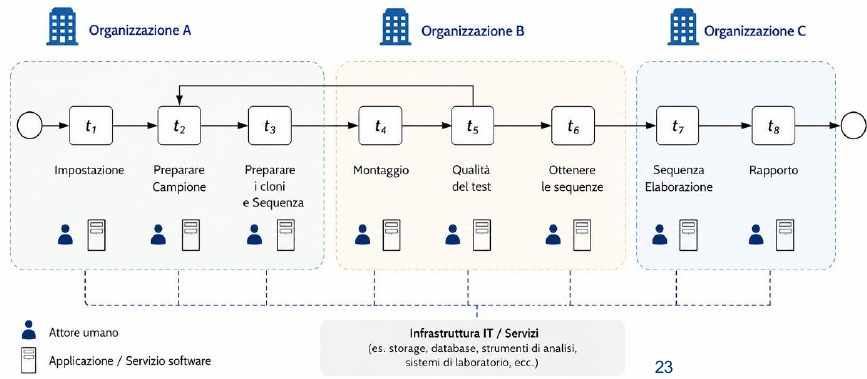
\includegraphics[scale=0.68]{figures/Schermata_20260513_121721.png}
\end{figure}

\subsection{Orchestrazione}
\subsubsection{Definizione}
Descrive come i servizi interagiscono tra loro, governati dalla \textbf{logica di business} e da un preciso \textbf{ordine di esecuzione} dal punto di vista e \uline{sotto il controllo di un singolo attore} (servizio orchestratore).
\subsubsection{Caratteristiche principali}
\begin{itemize}
    \item \textbf{Controllo centralizzato}: Un servizio orchestratore decide cosa succede e quando.
    \item \textbf{Gesione esplicita}: L'orchestratore conosce tutti i dettagli del flusso.
\end{itemize}
\subsubsection{Vantaggi}
\begin{itemize}
    \item Monitoraggio semplificato (tutto passa dall'orchestratore)
    \item Più facile gestire errori e transazioni
\end{itemize}
\subsubsection{Svantaggi}
\begin{itemize}
    \item Dipendenza dall'orchestratore.
    \item Accoppiamento più stretto tra servizi.
    \item Scalabilità limitata.
\end{itemize}
\subsubsection{Schema}
\begin{figure}[H]
    \centering
    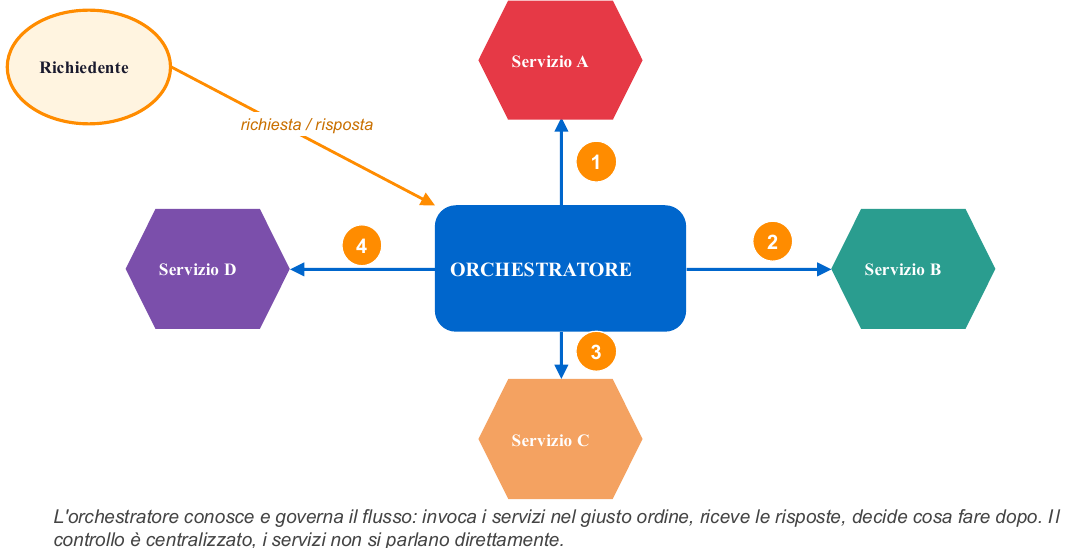
\includegraphics[scale=0.6]{figures/Schermata_20260513_122906.png}
\end{figure}

\newpage

\subsection{Coreografia}
\subsubsection{Definizione}
Descrive la sequenza di interazioni tra più parti coinvolte nel processo \textbf{dal punto di vista di tutte le parti}.

Definisce lo \uline{stato condiviso delle interazioni tra le entità}.

Ogni servizio è responsabile di portare a termine il proprio compito, invocando anche altri servizi.

Di solito viene implementato utilizzando eventi.
\subsubsection{Caratteristiche principali}
\begin{itemize}
    \item \textbf{Controllo distribuito}: Ogni servizio agisce autonomante.
    \item \textbf{Comunicazione tramite eventi}: Spesso i servizi reagiscono a eventi pubblicati da altri
\end{itemize}
\subsubsection{Vantaggi}
\begin{itemize}
    \item Alta scalabilità (ogni servizio è indipendente).
    \item Basso accoppiamento tra servizi.
    \item Resilienza (nessun single point of failure).
\end{itemize}
\subsubsection{Svantaggi}
\begin{itemize}
    \item Difficile da monitorare (flusso distribuito).
    \item Gestione errori complessa.
    \item Testing end-to-end più difficile.
\end{itemize}
\subsubsection{Schema}
\begin{figure}[H]
    \centering
    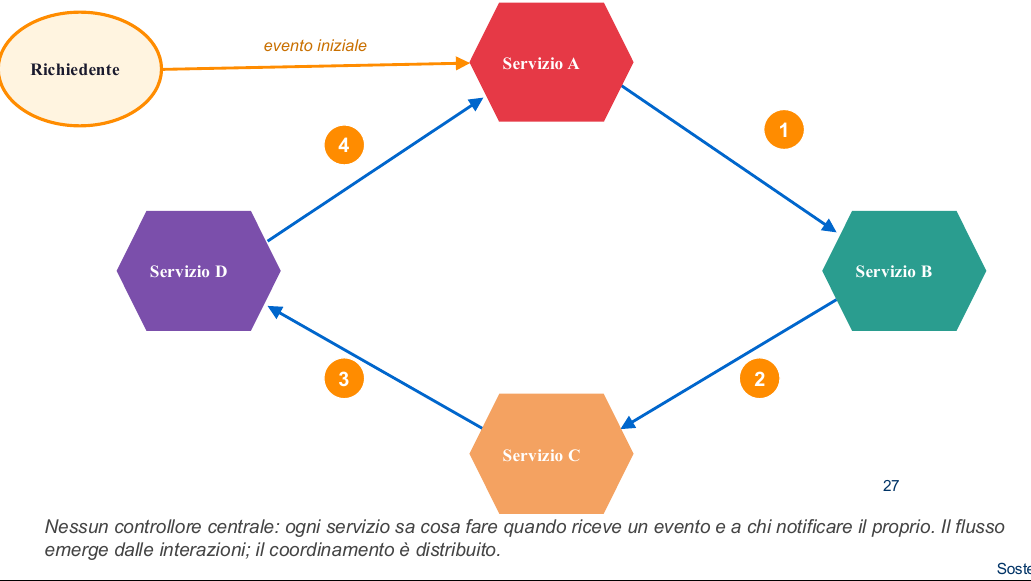
\includegraphics[scale=0.6]{figures/Schermata_20260513_134558.png}
\end{figure}

\section{Web API}
\subsection{Definizione}
Le Web API sono interfacce che permettono la comunicazione tra applicazioni software attraverso il web seguendo i principali come componenti indipendenti.

\subsection{Caratteristiche}
\begin{enumerate}
    \item \textbf{Interfaccia ben nota}
        \begin{itemize}
            \item Spesso supportata da un linguaggio di descrizione standard (WSDL o OpenAPI).
            \item Autoesplicativa: Include endpoints, metodi, parametri e risposte.
            \item Contratto di servizio: Definisce chiaramente le interazioni possibili.
            \item Possibile gestione automatica da parte del middleware.
        \end{itemize}
    \item \textbf{Punto di accesso unico}
        \begin{itemize}
            \item Indirizzabile tramite URI base:

            Il servizio ha un endpoint principale univoco.
            \item Scorpibile: Attraverso registri di servizi o discovery services.
            \item Gateway unificato: Singolo punto di ingresso per tutte le funzionalità di servizio.
        \end{itemize}
    \item \textbf{Scambio di dati basato su documenti}
        \begin{itemize}
            \item Utilizzo di un formato di rappresentazione standard.
            \item Usually stateless: Ogni richiesta contiene tutte le informazioni necessarie.
            \begin{tcolorbox}[breakable, title={Esempio: Risposta JSON da OpenWeatherMap API}]
                \begin{lstlisting}
{
    "temp": 22.5,
    "feels_like": 21.8,
    "humidity": 65,
    "wind_speed": 5.2
}
                \end{lstlisting}
            \end{tcolorbox}
        \end{itemize}
\end{enumerate}

\subsection{Esempio: openweathermaps}
Un semplice esempio di servizio web è un'API meteo.
\begin{itemize}
    \item \textbf{Identificato da un URI}:

    L'API meteo è accessibile tramite un URL.
    \item \textbf{Definita, descritta e scoperta}:

    L'API fornisce una documentazione che descrive le sue funzionalità, i parametri di input (come il nome della città o le coordinate) e gli output previsti (come la temperatura o le condizioni meteorologiche).
    \item \textbf{Supporta le interazioni attraverso i messaggi dei procotlli internet}:

    Le applicazioni comunicano con l'API meteo tramite \texttt{HTTP} o \texttt{HTTPS}.
    
    Ad esempio, un'applicazione può inviare una richiesta \texttt{GET} per recuperare i dati meteo attuali.
\end{itemize}

\begin{tcolorbox}[title={Esempio di interazione}, breakable]
    \begin{itemize}
        \item \textbf{Client Request}: \url{https://api.openweathermap.org/data/2.5/weather?q=Berlin&appid=your_api_key}
        \item \textbf{Server Response}: Dati in formato JSON contenuti informazioni meteo per Berlino, come ad esempio
        \begin{lstlisting}
{
  "weather": [{"description": "clear sky"}],
  "main": {"temp": 286.15},
  "name": "Berlin"
}
        \end{lstlisting}
    \end{itemize}
\end{tcolorbox}

\section{Operazioni di base in SOA}
L'interazione tra service provider, requestor e registry si articola in 3 operazioni fondamentali:
\begin{itemize}
    \item \textbf{Publish}

    Il provider pubblica nel registry la descrizione del proprio servizio (operazioni esposte, formati di input/output, endpoint).
    \item \textbf{Find}

    Il requestor interroga il registry alla ricerca di un servizio compatibile con le proprie esigenze, e ne ottiene la descrizione e l'endpoint.
    \item \textbf{Bind}/\textbf{Invoke}

    Il requestor stabilisce una connessione diretta con il provider e invoca il servizio (richiesta-risposta).
\end{itemize}
\begin{figure}[H]
    \centering
    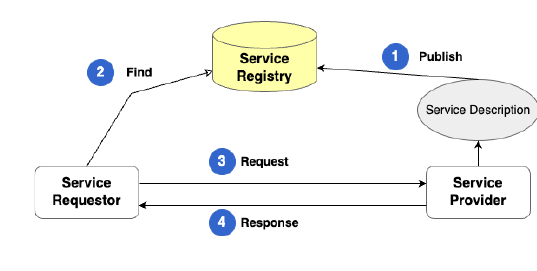
\includegraphics[scale=.72]{figures/Schermata_20260513_112300.png}
\end{figure}


Il registri partecipa solo alle prime 2 fasi: una volta ottenuto l'endpoint, requestor e provider comunicano direttamente.

È un ruolo passivo da catalogo.

\section{Comunicazione basata su broker}
\subsection{Definizione}
Nel modello classico il registry è passivo: indicizza i servizzi ma non partecipa all'invocazione.

Quando ai requiremetns si aggiungono \textbf{sicurezza, composizione, mediazione di protocollo o caching} il registry evolve in \textbf{Service Broker}: un intermediario attivo che si interpone in ogni interazione.

\begin{figure}[H]
    \centering
    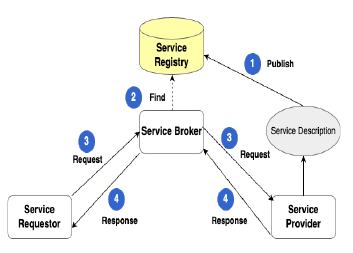
\includegraphics{figures/Schermata_20260513_113944.png}
\end{figure}

\subsection{Cosa cambio rispetto al registry?}
\begin{itemize}
    \item Le richieste passano \textbf{attraverso il broker}, non più direttamente al provider.
    \item Il broker può \textbf{autenticare, instradare, convertire} formati e protocolli, comporre più servizi in un'unica chiamata.
    \item Il \textbf{binding diventa dinamico}: il broker sceglie l'istanza del provider al momento della richiesta.
\end{itemize}

\subsection{Vantaggi}
\begin{itemize}
    \item \textbf{Disaccoppiamento}

    Provider e requestor non si conoscono direttamente, un provider può essere aggiornato senza impatto sui consumatori.
    \item \textbf{Interoperabilità}

    La mediazione permette a sistemi con protocolli diversi di dialogare.
    \item \textbf{Scalabilità}

    Il broker distribuisce il carico fra più istanze dello stesso servizio.
\end{itemize}

\newpage

\section{SLA - Service Level Agreement}
\subsection{Definizione informale}
Lo SLA definisce le modalità di erogazione di un servizio piuttosto che limitarsi a descrivere ciò che il servizio comporta.

\subsection{Definizione formale}
Un SLA è un contratto formalizzato che delinea gli standard, le aspettative e le metriche di prestazione concordate tra un fornitore di servizi e un consumatore di servizi.

\begin{figure}[H]
    \centering
    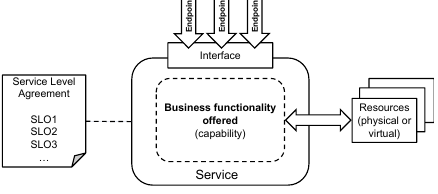
\includegraphics{figures/Schermata_20260513_120011.png}
\end{figure}

\subsection{Esempi di metriche SLA}
\begin{table}[h]
    \centering
    \renewcommand{\arraystretch}{1.5} % Spaziatura verticale per replicare l'altezza delle righe originale
    \begin{tabularx}{\textwidth}{|>{\bfseries}l|X|l|}
        \hline
        \textbf{Metric} & \textbf{Definition} & \textbf{Example Target} \\ \hline
        Availability & Percentage of time a service is operational. & 99.9\% per month. \\ \hline
        Response Time & Time to acknowledge a reported issue. & 15 minutes. \\ \hline
        Resolution Time & Time to resolve a critical incident. & 4 hours. \\ \hline
        Throughput & Volume of transactions processed per second. & 1,000 requests/sec. \\ \hline
        Error Rate & Percentage of failed transactions. & <1\% per month. \\ \hline
    \end{tabularx}
\end{table}

\section{Vantaggi e Svantaggi}
\subsection{Vantaggi}
\begin{itemize}
    \item Riutilizzabilità.
    \item Processo di sviluppo agile e orientato al business.
    \item Economia dei servizi.
    \item Scalabilità.
    \item Ottimizzazione e riduzione dei costi.
\end{itemize}
\subsection{Svantaggi}
\begin{itemize}
    \item Gestione del ciclo di vita complesso.
    \item Dependency Hell.
    \item Integrazione con le soluzioni legacy.
\end{itemize}

\chapter{SOAP - Simple Object Access Protocol}
\section{Definizione}
SOAP è un \textbf{protocollo di scambio messaggi basato su XML} che consente ad applicazioni software di comunicazione utilizzando messaggi XML.
\begin{itemize}
    \item Gli spazi dei nomi XML sono utilizzati per fornire una sementica ai dati (non solo ai tipi di dati)
    \item È agnostico rispetto al sottosistema di trasporto
    \item Permette di creare messaggi di richiesta e risposta in diverse configurazioni.
    \item Non è legato ad alcun linguaggio o piattaforma di programmazione (nemmeno ai servizi web)
    \item Utilizzato nei servizi orientati ai documenti
\end{itemize}

\section{Componenti di un messaggio SOAP}
\begin{figure}[H]
    \centering
    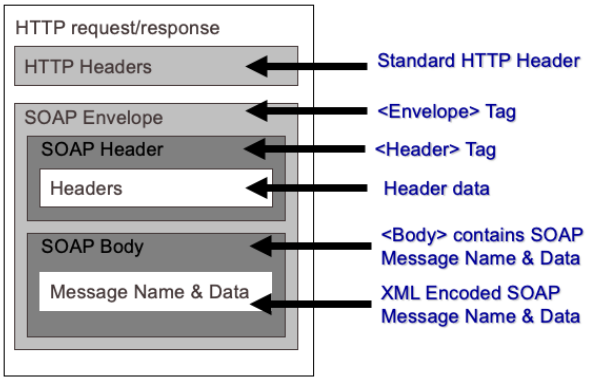
\includegraphics[scale=0.8]{figures/Schermata_20260513_135423.png}
\end{figure}

\newpage

\begin{itemize}
    \item \textbf{SOAP Envelope}
        \begin{itemize}
            \item Ingloba il contenuto del messaggio.
        \end{itemize}
    \item \textbf{SOAP Header (opzionale)}
        \begin{itemize}
            \item Maggiore flessibilità, può essere elaborato dai nodi tra l'origine e la destinazione.
            \item Contiene blocchi di informazioni su come elaborare il messaggio:
            
            \begin{itemize}
                \item Impostazione di instradamento e consegna.
                \item Asserzioni di autenticazione/autorizzazione.
                \item Contesti di transazione
            \end{itemize}
        \end{itemize}
    \item \textbf{SOAP Body}
        \begin{itemize}
            \item Messaggio effettivo da consegnare ed elaborare.
            \item Sia per le informazioni di richiesta che per quelle di risposta.
        \end{itemize}
\end{itemize}

\section{SOAP con HTTP}
Sebbene SOAP possa utilizzare diversi protocolli di trasporto, \texttt{HTTP} è quello più comunemente utilizzato.

\begin{itemize}
    \item Le richieste \texttt{HTTP} sono costituite da un metodo, come \texttt{POST} o \texttt{GET}, seguito dall'\texttt{URL} richiesto e dalla versione del protocollo.
    \item Le risposte seguono la semantica di \texttt{HTTP} per fornire il codice di stato della risposta.
\end{itemize}

\subsection{Modelli di scambio messaggi via HTTP}
Esistono due modelli per lo scambio di messaggi SOAP via \texttt{HTTP}:
\begin{itemize}
    \item Il modello \textbf{SOAP request-response} in cui il metodo \texttt{POST} viene utilizzato per portare i messaggi \texttt{SOAP} nel corpo delle richieste/risposte \texttt{HTTP}.

    \begin{tcolorbox}[breakable,title={Esempio di request-response}]
        \begin{lstlisting}[caption={Richiesta HTTP}]
POST /Reservations HTTP/1.1
Host: travelcompany.example.org
Content-Type: application/soap+xml; charset="utf-8"
Content-Length: 230

<?xml version='1.0' ?>
<env:Envelope xmlns:env="http://www.w3.org/2003/05/soap-envelope">
  <env:Header> ... </env:Header>
  <env:Body> ... </env:Body>
</env:Envelope>
        \end{lstlisting}
        \begin{lstlisting}[caption={Risposta HTTP}]
HTTP/1.1 200 OK
Content-Type: application/soap+xml; charset="utf-8"
Content-Length: 200
<?xml version='1.0' ?>
<env:Envelope
  xmlns:env="http://www.w3.org/2003/05/soap-envelope">
  <env:Header>...</env:Header>
  <env:Body>...</env:Body>
</env:Envelope>
        \end{lstlisting}
    \end{tcolorbox}
    \item Il modello \textbf{SOAP response} in cui nelle richieste \texttt{HTTP} viene utilizzato il metodo \texttt{GET} per ottenere il messaggio SOAP nel corpo della risposta.

    \begin{tcolorbox}[breakable, title={Esempio di response}]
        \begin{lstlisting}[caption={Richiesta HTTP}]
GET /travel.example.org/reservations?code=F3T HTTP/1.1
Host: travelcompany.example.org
Accept: text/html;q=0.5, application/soap+xml
        \end{lstlisting}
        \begin{lstlisting}[caption={Risposta HTTP}]
HTTP/1.1 200 OK
Content-Type: application/soap+xml; charset="utf-8"
Content-Length: 200
<?xml version='1.0' ?>
<env:Envelope
  xmlns:env="http://www.w3.org/2003/05/soap-envelope">
  <env:Header>...</env:Header>
  <env:Body>...</env:Body>
</env:Envelope>
        \end{lstlisting}
    \end{tcolorbox}
\end{itemize}

Utilizzando SOAP con \texttt{HTTP}, bisogna ricordarsi di impostare l'intestazione \textbf{\texttt{Content-Type}} come \textbf{\texttt{application/SOAP+xml}} 

\section{WSDL}
\subsection{Definizione}
WSDL è un linguaggi di descrizione dei servizi web basato su XML.

\subsection{Cosa descrive un documento WSDL}
WSDL consente di descrivere quattro dati principali per un servizio:
\begin{itemize}
    \item Infromazioni sull'\textbf{interfaccia} che descrivono tutte le operazioni pubblicamente disponibili di un servizio.
    \item Dichiarazioni di \textbf{tipi di dati} per tutti i messaggi.

    I tipi complessi possono essere dichiarati (utilizzando SOAP) e utilizzati.
    \item Informazioni di \textbf{binding} sul protocollo di trasporto.
    \item Informazioni sull'\textbf{indirizzo} per la localizzazione del servizio
\end{itemize}

\subsection{Modello concettuale}
\begin{figure}[H]
    \centering
    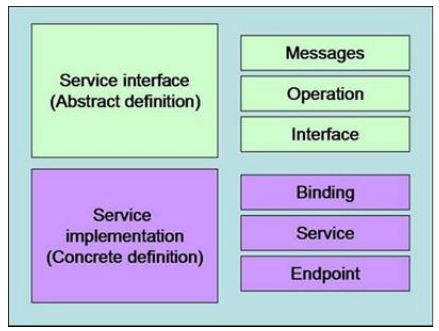
\includegraphics[scale=0.75]{figures/Schermata_20260514_092647.png}
\end{figure}
\begin{itemize}
    \item Nella parte \textbf{astratta}
    \begin{itemize}
        \item Descrizione di un servizio in termini di \textbf{messaggi} che invia e riceve attraverso un sistema di tipi, tipicamente \texttt{W3C XML Schema}
        \item Un'\textbf{operazione} associa \uline{modelli di scambio di messaggi} a uno o più messaggi.
        \item \textbf{I modelli di scambio di messaggi} definiscono la sequenza e la cardinalità dei messaggi scambiati tra i nodi (servizi).
        \item Un'\textbf{interfaccia} raggruppa queste operazioni in modo indipendente del canale di comunicazione.
    \end{itemize}
    \item Nella parte \textbf{concreta}
    \begin{itemize}
        \item I \textbf{binding} specificano il protocollo di trasporto per le interfacce.
        \item Un \textbf{endpoint} associa un \texttt{URI} a un binding.
        \item Un \textbf{servizio} ragruppa gli endpoint che implementano un'interfaccia comune.
    \end{itemize}
\end{itemize}

\subsection{Definizione del binding}


\begin{itemize}
    \item \textbf{Binding}:
    \begin{itemize}
    \item L'attributo \textbf{name} definisce il nome dei binding.

    Con questo nome si può fare riferimento ad esso quando si definisce un endpoint di servizio.
    \item Ogni nome di binding deve essere \uline{univoco all'interno dello spazio dei nomi del target \texttt{WSDL 2.0}}.
    \item L'attributo \textbf{interface} \uline{contiene il nome di una delle interfacce definite}.
    \item L'attributo \textbf{type} definisce il \uline{formato del messaggio} da utilizzare.

    In questo caso è SOAP.
    \item \textbf{\texttt{wsoap:protocol}} definisce il protocollo di "trasporto".

    Nell'esempio, i messaggi soap verrano trasportati utilizzando \texttt{HTTP}.
\end{itemize}
    \item \textbf{Operation}:
    \begin{itemize}
        \item L'attributo \textbf{ref} dell'elemento operation fa riferimento a una specifica operazione (già definita nella sezione interface).
        \item L'attributo \textbf{\texttt{wsoap:code}} dell'elemento fault definisce il codice di errore che determina l'invio di questo messaggio.
    \end{itemize}
    \item \textbf{Fault}:
    \begin{itemize}
        \item L'attributo \textbf{ref} definisce quale errore (già definito nella sezione dell'interfaccia) ci si riferisce per questo binding.
        \item L'attributo \textbf{\texttt{wsoap:code}} dell'elemento fault definisce il codice di errore che determina l'invio di questo messaggio.
    \end{itemize}
\end{itemize}

\begin{tcolorbox}[breakable,after title*={Esempio di binding}]
    \begin{lstlisting}
<binding name = "myServiceInterfacesOAPBinding"
         interface = "tns:myServiceInterface"
         type = "http://www.w3.org/ns/wsdl/soap"
         wsoap:protocol = "http://www.w3.org/2003/05/soap/bindings/HTTP/">
    <operation ref = "tns:checkServiceStatusOp"
               wsoap:mep = "http://www.w3.org/2003/05/soap/mep/soap-response/"/>
    <fault ref = "tns:dataFault"  wsoap:code = "soap:Sender"/>
</binding>
    \end{lstlisting}
\end{tcolorbox}

\subsection{Definizione di service/endpoint}
\begin{itemize}
    \item \textbf{Service}:
    \begin{itemize}
        \item L'attributo \textbf{name} definisce il nome del servizio.

        Ogni nome di servizio deve essere unico all'interno dello spazio dei nomi di destinazione.
        \item L'attributo \textbf{interface} definisce il nome dell'interfaccia (precedentemente definita nella sezione interface) implementanta dal servizio.
    \end{itemize}
    \item \textbf{Endpoint}:
    \begin{itemize}
        \item L'attributo \textbf{name} definisce il nome dell'endpoint, che deve essere unico all'interno dei servizi.
        \item L'attributo \textbf{binding} specifica quale binding già definito verrà utilizzato da questo endpoint.
        \item L'attributo \textbf{address} specifica l'indirizzo fisico dove il servizio sarà disponibile.
    \end{itemize}
\end{itemize}
\begin{tcolorbox}[breakable, title={Esempio di service/endpoint}]
    \begin{lstlisting}
<service name = "myService" interface = "tns: myServiceInterface">
    <endpoint name = "myServiceEndpoint"
              binding = "tns:myServiceInterfaceSOAPBinding"
              address = "http://yoursite.com/MyService"/>
</service>
    \end{lstlisting}
\end{tcolorbox}

\subsection{Declino di SOAP}
L'obbiettivo principale di SOAP era creare uno standard universale tra le applicazioni che fosse indipendente da piattaforme, linguaggi e protocolli di trasporto.

\subsubsection{Fattori di declino}
\begin{itemize}
    \item \textbf{Complessità eccessiva}:
    \begin{itemize}
        \item Struttura \texttt{XML} verbosa e rigida.
        \item Curve di apprendimento ripide.
        \item Costi di implementazione elevati
    \end{itemize}
    \item \textbf{Performance insufficienti}:
    \begin{itemize}
        \item Overhead significativo nella trasmissione dei dati.
        \item Parsing \texttt{XML} computazionale costoso.
        \item Latenza più elevata rispetto alle alternative
    \end{itemize}
    \item \textbf{Ascesa delle alternative}:
    \begin{itemize}
        \item \texttt{REST}: Più semplice, leggibile e veloce.
        \item \texttt{JSON}: Formato dati leggero e più facile da elaborare.
    \end{itemize}
\end{itemize}